\chapter[Interface SOC \& Visualisations]{Réalisation : Interface SOC, Cartographie \& Visualisations}
\label{chap:dashboard}

\section{Design System v2 « Digital Backbone »}
L'interface utilisateur de CyberScore TN a été pensée pour répondre aux standards esthétiques et ergonomiques des postes de commandement de cybersécurité modernes.

\subsection{Palette Chromatique \& Identité Visuelle}
L'ergonomie visuelle repose sur des contrastes élevés adaptés aux longues sessions de supervision :
\begin{itemize}
    \item \textbf{Fond Principal (\texttt{--bg-primary})} : Bleu nuit profond (\texttt{\#04151f}) éliminant la fatigue oculaire.
    \item \textbf{Cartes \& Panneaux (\texttt{--bg-secondary})} : Surface bleu acier sombre (\texttt{\#0a2233}) avec effet de glassmorphism subtil (\texttt{backdrop-filter: blur(8px)}).
    \item \textbf{Accent Principal (\texttt{--color-primary})} : Cyan électrique (\texttt{\#00e5ff}) pour les éléments actifs et trajectoires.
    \item \textbf{Codes de Sévérité Universels} : Vert émeraude (\texttt{\#00e676}) pour les postures excellentes, ambre (\texttt{\#ffb300}) pour les alertes modérées, et rouge écarlate (\texttt{\#ff1744}) pour les failles critiques.
\end{itemize}

\section{Centre de Commande National (Command Center)}
Le Command Center (\texttt{/}) rassemble l'ensemble des flux télémétriques de l'État :
\begin{enumerate}
    \item \textbf{StatCards Connectées en Temps Réel} : Affichage dynamique des quatre indicateurs clés de performance : nombre d'institutions sous surveillance active (121 sites gouvernementaux), score moyen national consolidé (57.6/100), alertes critiques réelles détectées (112) et volume des scans effectués dans la journée.
    \item \textbf{Leaderboard National \& Modal d'Aperçu Interactif} : Tableau de classement trié par note. Un clic sur n'importe quel organisme ouvre instantanément une visionneuse interactive de 7 pages (\texttt{ReportPreviewModal.tsx}) affichant la synthèse exécutive, l'analyse radar et les vulnérabilités détectées.
\end{enumerate}

\subsection{Recalibrage Géométrique SVG de la Carte de Tunisie}
L'affichage cartographique régional présentait initialement un rognage sur le gouvernorat de Tataouine et les côtes de Djerba. Une analyse trigonométrique des coordonnées des 24 gouvernorats a permis d'établir l'emprise géographique réelle :
\begin{itemize}
    \item \textbf{Axe horizontal} : De $X = 289.5$ (Tozeur / frontière ouest) à $X = 710.5$ (Djerba / côtes est), soit une largeur de 421.0 px.
    \item \textbf{Axe vertical} : De $Y = 45.5$ (Bizerte / Cap Blanc) à $Y = 954.5$ (Borj El Khadra / pointe sud), soit une hauteur de 909.0 px.
\end{itemize}
Le composant vectoriel SVG a été calibré avec la \texttt{viewBox} optimale :
\begin{lstlisting}[language=XML, caption={Recalibrage du composant vectoriel de la carte de Tunisie}]
<svg id="tn-map" viewBox="275 35 450 935" xmlns="http://www.w3.org/2000/svg">
\end{lstlisting}
Chaque gouvernorat est coloré dynamiquement en fonction du score moyen des sites rattachés à sa circonscription administrative (Figure \ref{fig:dashboard_view}).

\begin{figure}[!htbp]
\centering
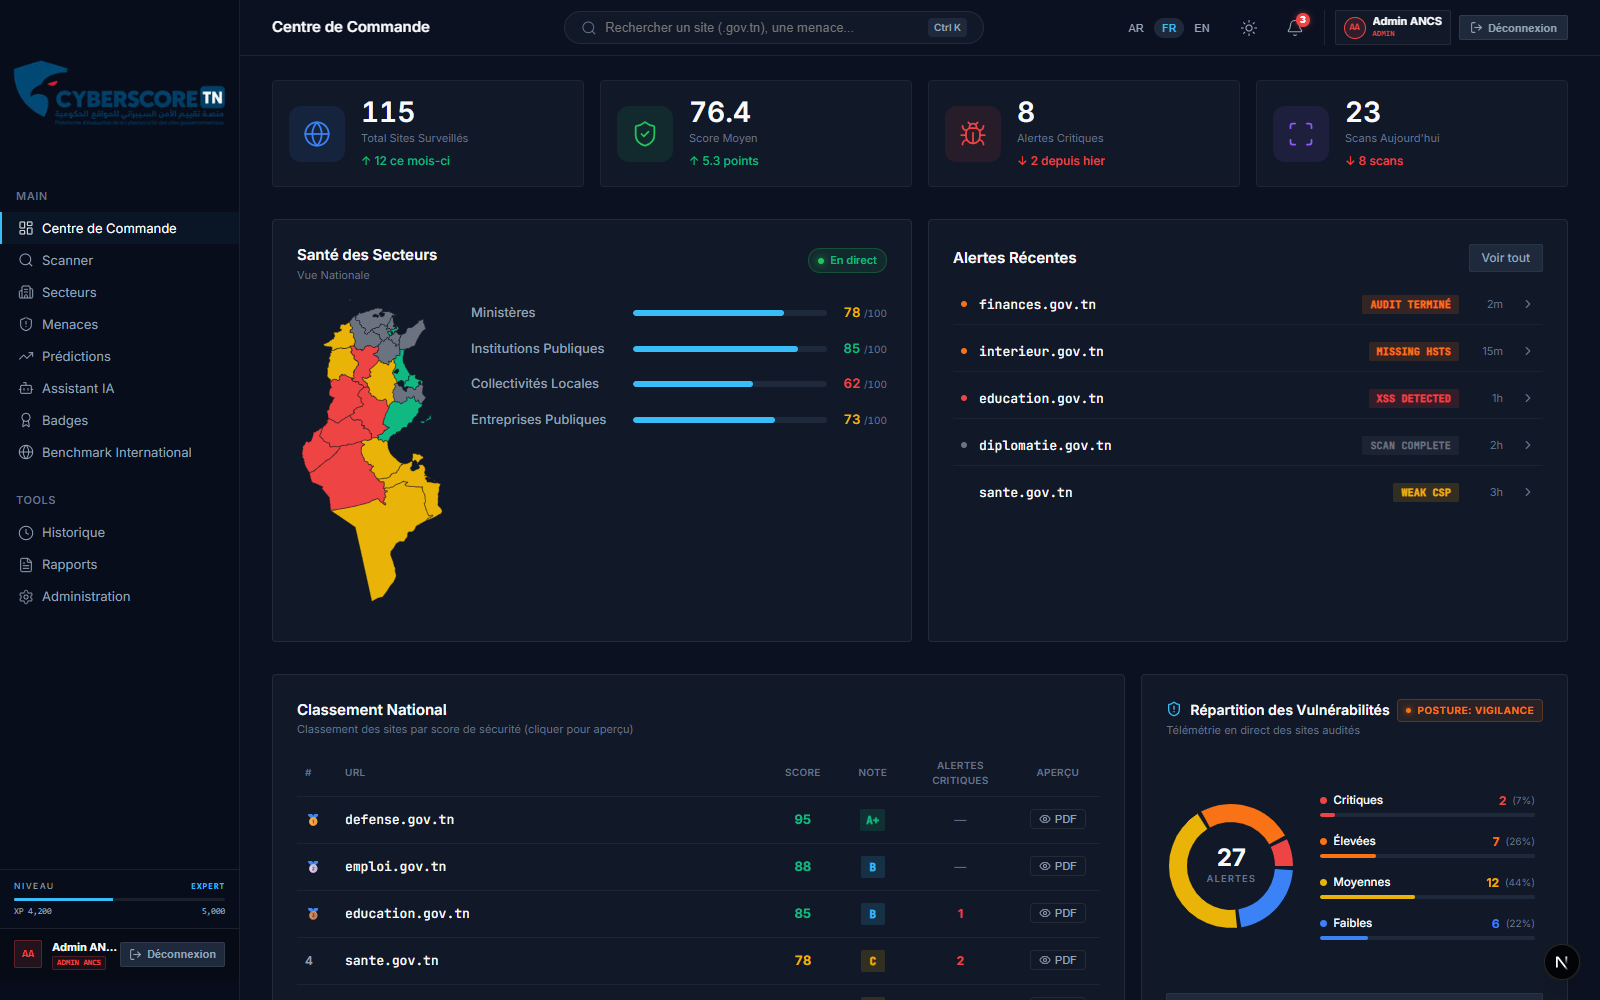
\includegraphics[width=0.70\textwidth]{images/dashboard.png}
\caption{Tableau de bord national (Command Center) et cartographie vectorielle interactive}
\label{fig:dashboard_view}
\end{figure}

\section{Observatoire de Benchmark International \& Étalonnage (\texttt{/benchmark})}
L'Observatoire International permet de situer la posture nationale de la Tunisie par rapport aux standards mondiaux et aux pays pairs de la région MENA et d'Europe :
\begin{itemize}
    \item \textbf{Calcul Dynamique en Temps Réel} : Contrairement aux approches statiques, la position de la Tunisie est recalculée dynamiquement à partir des audits réels des 121 portails gouvernementaux et des scans interactifs.
    \item \textbf{Étalonnage par Piliers Techniques} : Comparaison fine sur six axes cruciaux : chiffrement SSL/TLS, en-têtes HTTP de sécurité, sécurité DNS/DNSSEC, exposition des ports réseau, politique de cookies et Content Security Policy (CSP).
    \item \textbf{Synchronisation Réactive} : Tout audit réalisé dans le scanner met instantanément à jour le score national et le classement comparatif.
\end{itemize}

\section{War Room \& Mappemonde Cyber Animée (\texttt{/threats})}
La page de surveillance des cybermenaces propose une tour de contrôle combinant audits réels et télémétrie mondiale (CTI) :
\begin{itemize}
    \item \textbf{Moteur Graphique Canvas 60 FPS} : Rendu fluide affichant les trajectoires balistiques d'attaques mondiales modélisées par des courbes de Bézier quadratiques convergeant vers les coordonnées géographiques de la Tunisie (33.88\textdegree{} N, 9.53\textdegree{} E).
    \item \textbf{Effets d'Impact \& Détection de Collision} : Les flux interceptés par les pare-feu périmétriques déclenchent un flash visuel au point d'impact.
    \item \textbf{Cartes Hybrides des Vulnérabilités (CVEs)} : Affichage prioritaire des failles critiques réelles identifiées lors des scans de nos serveurs étatiques, complété par un flux de renseignement mondial sur les menaces émergentes.
\end{itemize}

\begin{figure}[!htbp]
\centering
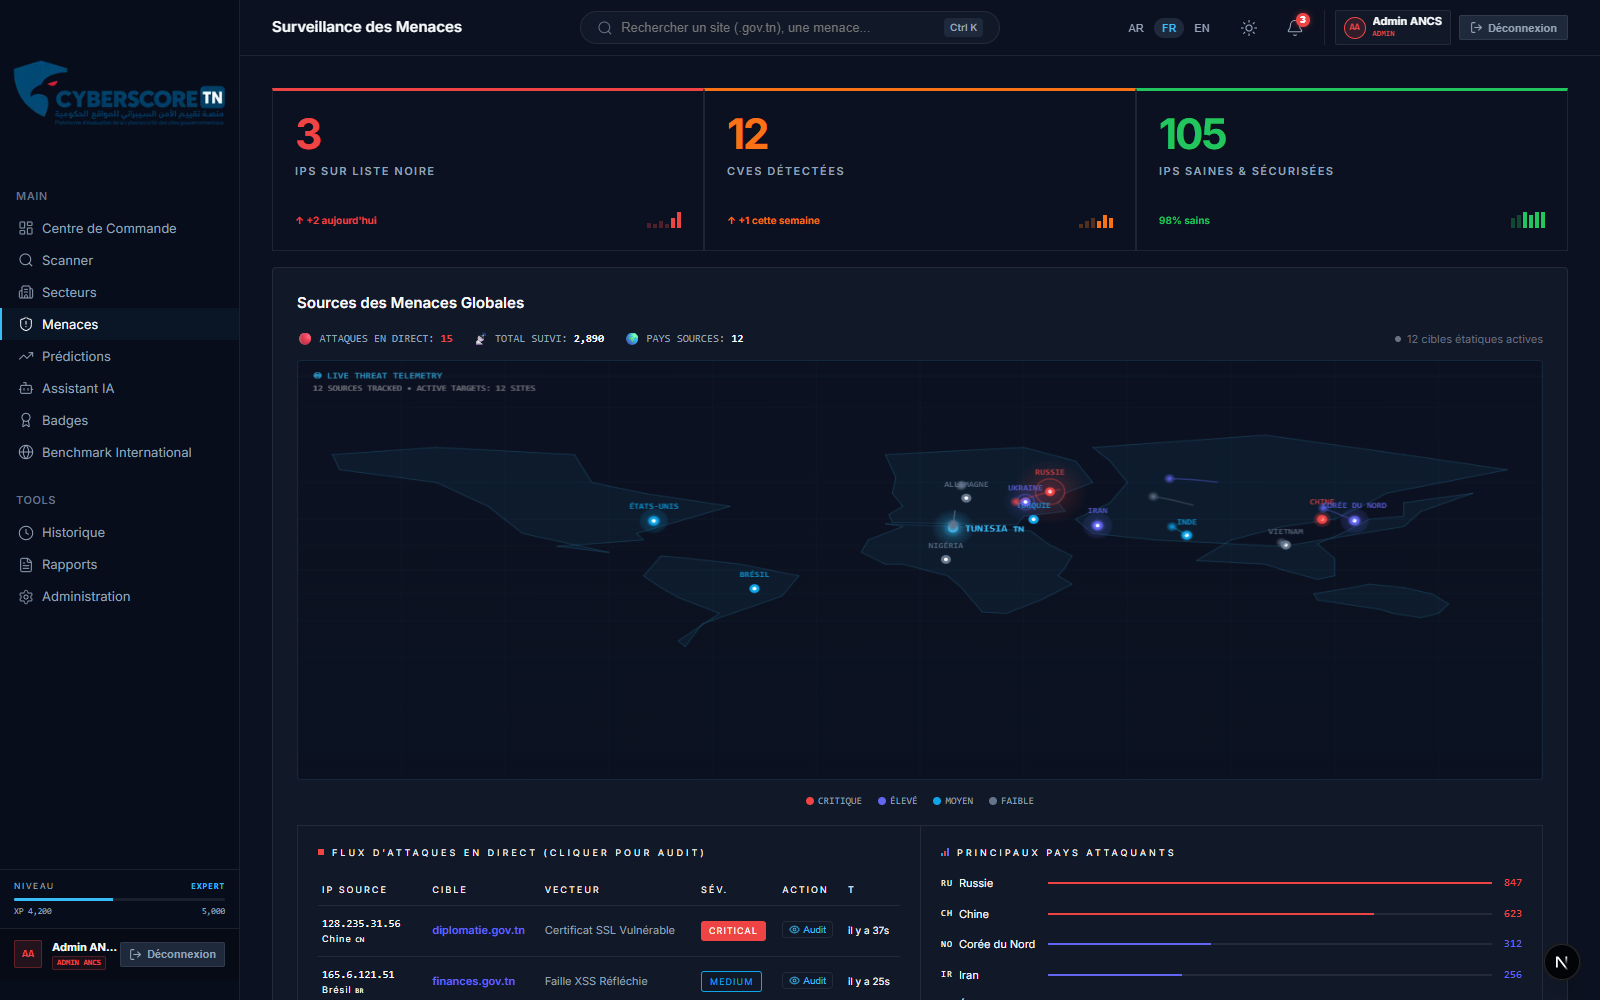
\includegraphics[width=0.70\textwidth]{images/threats.png}
\caption{War Room souveraine et flux mondial des cyberattaques en temps réel (Canvas 60 FPS)}
\label{fig:threats_view}
\end{figure}

\section{Centre National d'Édition des Rapports d'Audit (\texttt{/reports})}
Le module de reporting certifié permet d'exporter des fiches d'audit et des attestations officielles au format PDF vectoriel haute résolution. Chaque rapport intègre :
\begin{itemize}
    \item \textbf{Cartouche Officiel de Conformité ANCS} : Mention du Décret-loi n° 2023-17 et classification TLP.
    \item \textbf{Visualisation Radar des 16 Piliers} : Graphique vectoriel A4 illustrant la posture technique relative.
    \item \textbf{Signature Numérique SHA-256 \& QR Code} : Empreinte cryptographique certifiant l'intégrité du document sans altération (Figure \ref{fig:reports_view}).
\end{itemize}

\begin{figure}[!htbp]
\centering
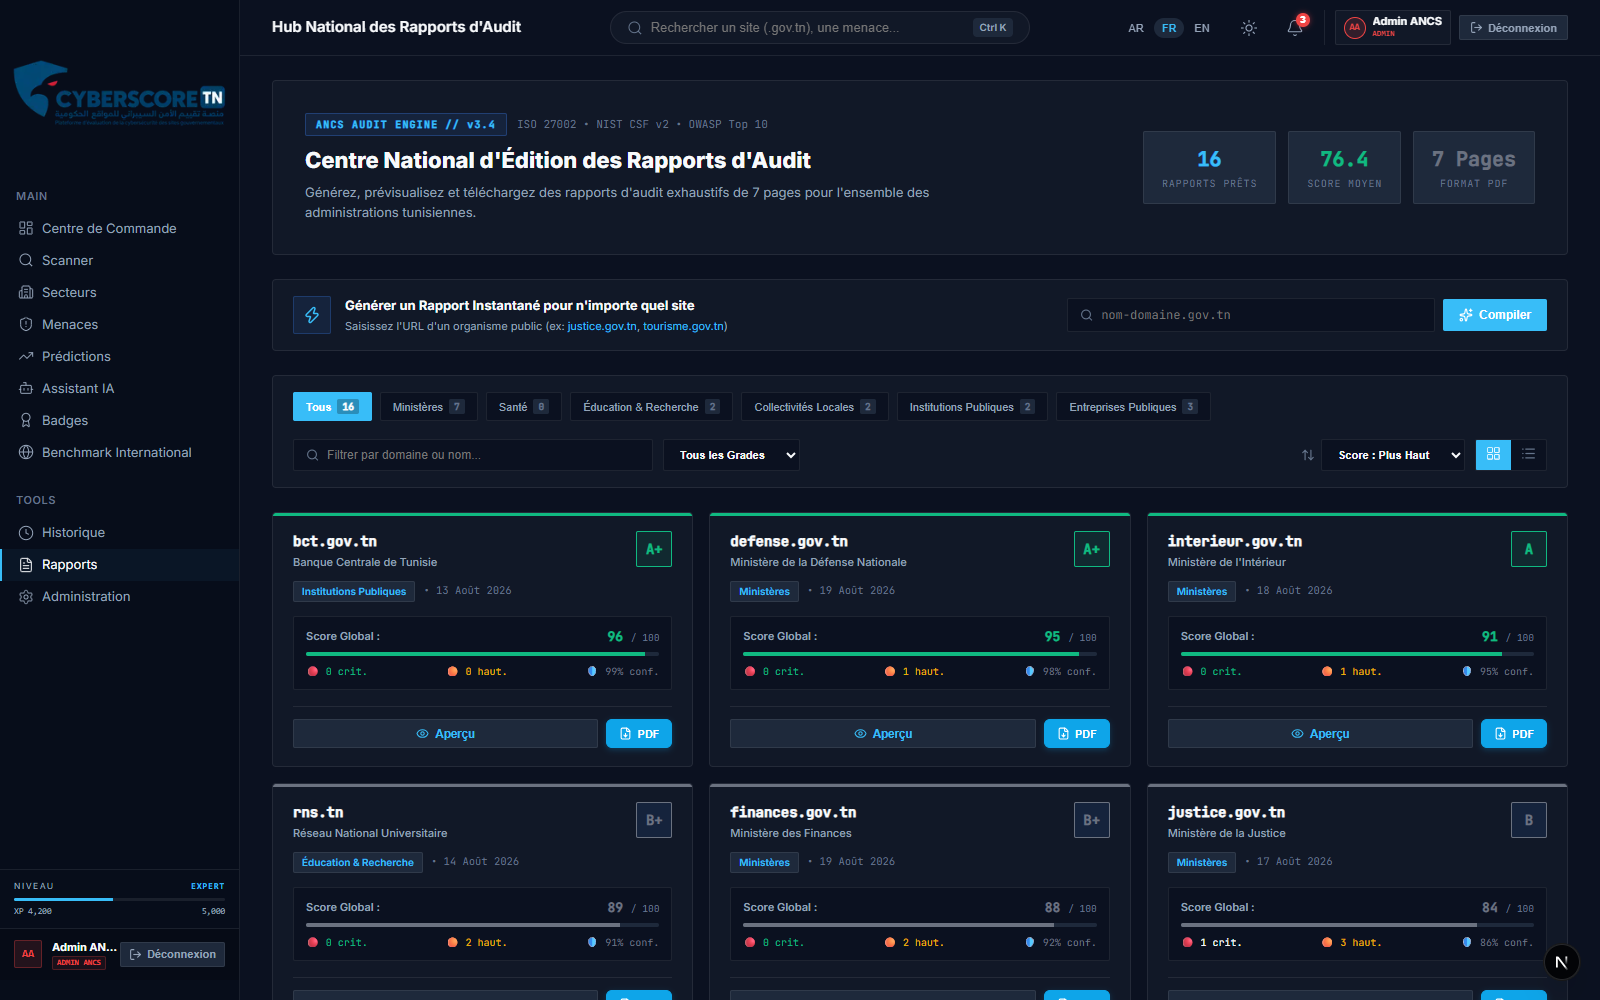
\includegraphics[width=0.70\textwidth]{images/reports.png}
\caption{Centre d'édition des rapports d'audit officiels et d'attestations de conformité}
\label{fig:reports_view}
\end{figure}
